\documentclass[12pt,letterpaper]{article}\usepackage[]{graphicx}\usepackage[]{color}
%% maxwidth is the original width if it is less than linewidth
%% otherwise use linewidth (to make sure the graphics do not exceed the margin)
\makeatletter
\def\maxwidth{ %
  \ifdim\Gin@nat@width>\linewidth
    \linewidth
  \else
    \Gin@nat@width
  \fi
}
\makeatother

\definecolor{fgcolor}{rgb}{0.345, 0.345, 0.345}
\newcommand{\hlnum}[1]{\textcolor[rgb]{0.686,0.059,0.569}{#1}}%
\newcommand{\hlstr}[1]{\textcolor[rgb]{0.192,0.494,0.8}{#1}}%
\newcommand{\hlcom}[1]{\textcolor[rgb]{0.678,0.584,0.686}{\textit{#1}}}%
\newcommand{\hlopt}[1]{\textcolor[rgb]{0,0,0}{#1}}%
\newcommand{\hlstd}[1]{\textcolor[rgb]{0.345,0.345,0.345}{#1}}%
\newcommand{\hlkwa}[1]{\textcolor[rgb]{0.161,0.373,0.58}{\textbf{#1}}}%
\newcommand{\hlkwb}[1]{\textcolor[rgb]{0.69,0.353,0.396}{#1}}%
\newcommand{\hlkwc}[1]{\textcolor[rgb]{0.333,0.667,0.333}{#1}}%
\newcommand{\hlkwd}[1]{\textcolor[rgb]{0.737,0.353,0.396}{\textbf{#1}}}%

\usepackage{framed}
\makeatletter
\newenvironment{kframe}{%
 \def\at@end@of@kframe{}%
 \ifinner\ifhmode%
  \def\at@end@of@kframe{\end{minipage}}%
  \begin{minipage}{\columnwidth}%
 \fi\fi%
 \def\FrameCommand##1{\hskip\@totalleftmargin \hskip-\fboxsep
 \colorbox{shadecolor}{##1}\hskip-\fboxsep
     % There is no \\@totalrightmargin, so:
     \hskip-\linewidth \hskip-\@totalleftmargin \hskip\columnwidth}%
 \MakeFramed {\advance\hsize-\width
   \@totalleftmargin\z@ \linewidth\hsize
   \@setminipage}}%
 {\par\unskip\endMakeFramed%
 \at@end@of@kframe}
\makeatother

\definecolor{shadecolor}{rgb}{.97, .97, .97}
\definecolor{messagecolor}{rgb}{0, 0, 0}
\definecolor{warningcolor}{rgb}{1, 0, 1}
\definecolor{errorcolor}{rgb}{1, 0, 0}
\newenvironment{knitrout}{}{} % an empty environment to be redefined in TeX

\usepackage{alltt}
 \usepackage[left=2cm,right=2cm,top=2cm,bottom=2cm]{geometry}
\usepackage[ansinew]{inputenc}
\usepackage[spanish]{babel}
\usepackage{amsmath}
\usepackage{amsfonts}
\usepackage{amssymb}
\usepackage{dsfont}
\usepackage{multicol} 
\usepackage{subfigure}
\usepackage{graphicx}
\usepackage{float} 
\usepackage{verbatim} 
\usepackage[left=2cm,right=2cm,top=2cm,bottom=2cm]{geometry}
\usepackage{fancyhdr}
\pagestyle{fancy} 
\fancyhead[LO]{\leftmark}
\usepackage{caption}
\newtheorem{definicion}{Definci\'on}
\IfFileExists{upquote.sty}{\usepackage{upquote}}{}
\begin{document}

\begin{titlepage}
\setlength{\unitlength}{1 cm} %Especificar unidad de trabajo


\begin{center}
\textbf{{\large UNIVERSIDAD DE EL SALVADOR}\\
{\large FACULTAD MULTIDISCIPLINARIA DE OCCIDENTE}\\
{\large DEPARTAMENTO DE MATEM\'ATICA}}\\[0.50 cm]

\begin{picture}(18,4)
 \put(7,0){
\includegraphics[width=4cm]{minerva.jpg}}
\end{picture}
\\[0.25 cm]

\textbf{{\large Licenciatura en Estad\'istica}\\[1.25cm]
{\large Control Estadistico del Paquete R }\\[2 cm]
%\setlength{\unitlength}{1 cm}
{\large  \textbf{''UNIDAD DOS"}}\\
{\large  \textbf{PR\'ACTICA 08}}\\[3 cm]
{\large Alumna:}\\
{\large Erika Beatr\'i Guill\'en Pineda}\\ [2cm]
{\large Fecha de elaboraci\'on}\\
Santa Ana - \today }
\end{center}
\end{titlepage}

\newtheorem{teorema}{Teorema}
\newtheorem{prop}{Proposici\'on}[section]


\chead{PR\'ACTICA 08}
\cfoot{UESOCC}
\rfoot{\thepage}
%\pagestyle{fancy} 

\setcounter{page}{1}
\newpage




\section{AN\'ALISIS ESTAD\'ISTICO DE LOS DATOS. }


\begin{enumerate}
  
\item Visualiza el directorio por defecto y activa su directorio de trabajo
\begin{knitrout}
\definecolor{shadecolor}{rgb}{0.969, 0.969, 0.969}\color{fgcolor}\begin{kframe}
\begin{alltt}
\hlkwd{getwd}\hlstd{()}
\end{alltt}
\begin{verbatim}
## [1] "C:/Users/User/Documents/TODAS_PRACTICAS"
\end{verbatim}
\begin{alltt}
\hlkwd{setwd}\hlstd{(}\hlstr{"C:/Users/User/Documents/TODAS_PRACTICAS"}\hlstd{)}
\end{alltt}
\end{kframe}
\end{knitrout}

\item Crea un nuevo Script y ll\'amale "Script08-DatosContinuos" 

\item  Crea el vector que contendr\'a los datos.
\begin{knitrout}
\definecolor{shadecolor}{rgb}{0.969, 0.969, 0.969}\color{fgcolor}\begin{kframe}
\begin{alltt}
\hlstd{Notas} \hlkwb{<-} \hlkwd{c}\hlstd{(}\hlnum{4.47}\hlstd{,} \hlnum{4.47}\hlstd{,} \hlnum{3.48}\hlstd{,} \hlnum{5.0}\hlstd{,} \hlnum{3.42}\hlstd{,} \hlnum{3.78}\hlstd{,} \hlnum{3.1}\hlstd{,} \hlnum{3.57}\hlstd{,} \hlnum{4.2}\hlstd{,} \hlnum{4.5}\hlstd{,} \hlnum{3.6}\hlstd{,}
           \hlnum{3.75}\hlstd{,}  \hlnum{4.5}\hlstd{,}  \hlnum{2.85}\hlstd{,}  \hlnum{3.7}\hlstd{,}  \hlnum{4.2}\hlstd{,}  \hlnum{3.2}\hlstd{,}  \hlnum{4.05}\hlstd{,}  \hlnum{4.9}\hlstd{,}  \hlnum{5.1}\hlstd{,} \hlnum{5.3}\hlstd{,}
           \hlnum{4.16}\hlstd{,} \hlnum{4.56}\hlstd{,} \hlnum{3.54}\hlstd{,} \hlnum{3.5}\hlstd{,} \hlnum{5.2}\hlstd{,} \hlnum{4.71}\hlstd{,} \hlnum{3.7}\hlstd{,} \hlnum{4.78}\hlstd{,} \hlnum{4.14}\hlstd{,} \hlnum{4.14}\hlstd{,} \hlnum{4.8}\hlstd{,}
           \hlnum{4.1}\hlstd{,} \hlnum{3.83}\hlstd{,} \hlnum{3.6}\hlstd{,} \hlnum{2.98}\hlstd{,} \hlnum{4.32}\hlstd{,} \hlnum{5.1}\hlstd{,} \hlnum{4.3}\hlstd{,} \hlnum{3.9}\hlstd{,} \hlnum{3.96}\hlstd{,} \hlnum{3.54}\hlstd{,} \hlnum{4.8}\hlstd{,}
           \hlnum{4.3}\hlstd{,}  \hlnum{3.39}\hlstd{,} \hlnum{4.47}\hlstd{,} \hlnum{3.19}\hlstd{,} \hlnum{3.75}\hlstd{,} \hlnum{3.1}\hlstd{,}  \hlnum{4.7}\hlstd{,} \hlnum{3.69}\hlstd{,} \hlnum{3.3}\hlstd{,}  \hlnum{2.85}\hlstd{,}
           \hlnum{5.25}\hlstd{,} \hlnum{4.68}\hlstd{,} \hlnum{4.04}\hlstd{,} \hlnum{4.44}\hlstd{,} \hlnum{5.43}\hlstd{,} \hlnum{3.04}\hlstd{,} \hlnum{2.95}\hlstd{); Notas}
\end{alltt}
\begin{verbatim}
##  [1] 4.47 4.47 3.48 5.00 3.42 3.78 3.10 3.57 4.20 4.50 3.60 3.75 4.50 2.85
## [15] 3.70 4.20 3.20 4.05 4.90 5.10 5.30 4.16 4.56 3.54 3.50 5.20 4.71 3.70
## [29] 4.78 4.14 4.14 4.80 4.10 3.83 3.60 2.98 4.32 5.10 4.30 3.90 3.96 3.54
## [43] 4.80 4.30 3.39 4.47 3.19 3.75 3.10 4.70 3.69 3.30 2.85 5.25 4.68 4.04
## [57] 4.44 5.43 3.04 2.95
\end{verbatim}
\begin{alltt}
\hlkwd{data.entry}\hlstd{(Notas)}
\hlstd{Notas}
\end{alltt}
\begin{verbatim}
##  [1] 4.47 4.47 3.48 5.00 3.42 3.78 3.10 3.57 4.20 4.50 3.60 3.75 4.50 2.85
## [15] 3.70 4.20 3.20 4.05 4.90 5.10 5.30 4.16 4.56 3.54 3.50 5.20 4.71 3.70
## [29] 4.78 4.14 4.14 4.80 4.10 3.83 3.60 2.98 4.32 5.10 4.30 3.90 3.96 3.54
## [43] 4.80 4.30 3.39 4.47 3.19 3.75 3.10 4.70 3.69 3.30 2.85 5.25 4.68 4.04
## [57] 4.44 5.43 3.04 2.95
\end{verbatim}
\begin{alltt}
\hlkwd{length}\hlstd{(Notas)}
\end{alltt}
\begin{verbatim}
## [1] 60
\end{verbatim}
\end{kframe}
\end{knitrout}

\item Guarda el vector de datos en un archivo.
\begin{knitrout}
\definecolor{shadecolor}{rgb}{0.969, 0.969, 0.969}\color{fgcolor}\begin{kframe}
\begin{alltt}
\hlkwd{write}\hlstd{(Notas,} \hlstr{"Notas.txt"}\hlstd{)}
\end{alltt}
\end{kframe}
\end{knitrout}

\item  Limpia el \'area de trabajo (Workspace)
\begin{knitrout}
\definecolor{shadecolor}{rgb}{0.969, 0.969, 0.969}\color{fgcolor}\begin{kframe}
\begin{alltt}
\hlkwd{ls}\hlstd{()}
\end{alltt}
\begin{verbatim}
## [1] "Notas"
\end{verbatim}
\begin{alltt}
\hlkwd{rm}\hlstd{(}\hlkwc{list}\hlstd{=}\hlkwd{ls}\hlstd{(}\hlkwc{all}\hlstd{=}\hlnum{TRUE}\hlstd{))}
\hlkwd{ls}\hlstd{()}
\end{alltt}
\begin{verbatim}
## character(0)
\end{verbatim}
\end{kframe}
\end{knitrout}

\item  Lee o recupera el vector de datos desde el archivo de texto. 
\begin{knitrout}
\definecolor{shadecolor}{rgb}{0.969, 0.969, 0.969}\color{fgcolor}\begin{kframe}
\begin{alltt}
\hlstd{X} \hlkwb{<-} \hlkwd{scan}\hlstd{(}\hlstr{"Notas.txt"}\hlstd{,} \hlkwc{what} \hlstd{=} \hlkwd{double}\hlstd{(}\hlnum{0}\hlstd{),} \hlkwc{na.strings} \hlstd{=} \hlstr{"NA"}\hlstd{,} \hlkwc{flush}\hlstd{=}\hlnum{FALSE}\hlstd{)}
\hlkwd{ls}\hlstd{()}
\end{alltt}
\begin{verbatim}
## [1] "X"
\end{verbatim}
\begin{alltt}
\hlcom{# Si el vector contiene valores reales se ocupa:}

\hlstd{what} \hlkwb{=} \hlkwd{double}\hlstd{(}\hlnum{0}\hlstd{)}
\end{alltt}
\end{kframe}
\end{knitrout}

\item Crea la tabla de frecuencias.
\begin{knitrout}
\definecolor{shadecolor}{rgb}{0.969, 0.969, 0.969}\color{fgcolor}\begin{kframe}
\begin{alltt}
\hlcom{# Define el numero k de los intervalos o clases. }

\hlcom{# Usa el Metodo de Herbert A. Sturges para determinar dicho numero.}

\hlstd{n} \hlkwb{<-} \hlkwd{length}\hlstd{(X); n}
\end{alltt}
\begin{verbatim}
## [1] 60
\end{verbatim}
\begin{alltt}
\hlstd{k} \hlkwb{<-} \hlnum{1}\hlopt{+}\hlnum{3.322}\hlopt{*}\hlkwd{logb}\hlstd{(n,} \hlnum{10}\hlstd{); k}
\end{alltt}
\begin{verbatim}
## [1] 6.907018
\end{verbatim}
\begin{alltt}
\hlstd{k} \hlkwb{<-} \hlkwd{round}\hlstd{(k); k}
\end{alltt}
\begin{verbatim}
## [1] 7
\end{verbatim}
\end{kframe}
\end{knitrout}

\begin{knitrout}
\definecolor{shadecolor}{rgb}{0.969, 0.969, 0.969}\color{fgcolor}\begin{kframe}
\begin{alltt}
\hlcom{# Calcula el ancho o amplitud a de cada intervalo a=rango/k}

\hlstd{rango} \hlkwb{<-} \hlkwd{max}\hlstd{(X)}\hlopt{-}\hlkwd{min}\hlstd{(X); rango}
\end{alltt}
\begin{verbatim}
## [1] 2.58
\end{verbatim}
\begin{alltt}
\hlstd{a}\hlkwb{=}\hlstd{rango}\hlopt{/}\hlstd{k; a}
\end{alltt}
\begin{verbatim}
## [1] 0.3685714
\end{verbatim}
\begin{alltt}
\hlstd{a} \hlkwb{<-} \hlkwd{round}\hlstd{(a,} \hlnum{3}\hlstd{); a}
\end{alltt}
\begin{verbatim}
## [1] 0.369
\end{verbatim}
\end{kframe}
\end{knitrout}

\begin{knitrout}
\definecolor{shadecolor}{rgb}{0.969, 0.969, 0.969}\color{fgcolor}\begin{kframe}
\begin{alltt}
\hlcom{# Define los limites y puntos mediosde cada uno de los k intervalos}

\hlstd{limites} \hlkwb{<-} \hlkwd{c}\hlstd{(}\hlkwc{from} \hlstd{=} \hlkwd{min}\hlstd{(X)}\hlopt{-}\hlnum{0.01}\hlopt{/}\hlnum{2}\hlstd{,} \hlkwc{to} \hlstd{=} \hlkwd{max}\hlstd{(X)}\hlopt{+}\hlnum{0.01}\hlopt{/}\hlnum{2}\hlstd{,} \hlkwc{by}\hlstd{=a); limites}
\end{alltt}
\begin{verbatim}
##  from    to    by 
## 2.845 5.435 0.369
\end{verbatim}
\begin{alltt}
\hlkwd{options}\hlstd{(}\hlkwc{digits}\hlstd{=}\hlnum{4}\hlstd{)}
\end{alltt}
\end{kframe}
\end{knitrout}

\begin{knitrout}
\definecolor{shadecolor}{rgb}{0.969, 0.969, 0.969}\color{fgcolor}\begin{kframe}
\begin{alltt}
\hlstd{ci} \hlkwb{<-} \hlkwd{cbind}\hlstd{(}\hlnum{1}\hlopt{:}\hlstd{k); ci}
\end{alltt}
\begin{verbatim}
##      [,1]
## [1,]    1
## [2,]    2
## [3,]    3
## [4,]    4
## [5,]    5
## [6,]    6
## [7,]    7
\end{verbatim}
\begin{alltt}
\hlkwa{for}\hlstd{(i} \hlkwa{in} \hlnum{2}\hlopt{:}\hlkwd{length}\hlstd{(limites)) ci[i}\hlopt{-}\hlnum{1}\hlstd{,} \hlnum{1}\hlstd{]} \hlkwb{<-} \hlstd{(limites[i]}\hlopt{+} \hlstd{limites[i}\hlopt{-}\hlnum{1}\hlstd{])}\hlopt{/}\hlnum{2}

\hlstd{ci}
\end{alltt}
\begin{verbatim}
##       [,1]
## [1,] 4.140
## [2,] 2.902
## [3,] 3.000
## [4,] 4.000
## [5,] 5.000
## [6,] 6.000
## [7,] 7.000
\end{verbatim}
\end{kframe}
\end{knitrout}

\begin{knitrout}
\definecolor{shadecolor}{rgb}{0.969, 0.969, 0.969}\color{fgcolor}\begin{kframe}
\begin{alltt}
\hlcom{# Encuentra las frecuencias absolutas fi para cada intervalo.}

\hlkwd{options}\hlstd{(}\hlkwc{digits}\hlstd{=}\hlnum{2}\hlstd{)}
\hlstd{fi} \hlkwb{<-} \hlkwd{cbind}\hlstd{(}\hlkwd{table}\hlstd{(}\hlkwd{cut}\hlstd{(X,} \hlkwc{breaks} \hlstd{= limites,} \hlkwc{labels}\hlstd{=}\hlkwa{NULL}\hlstd{,} \hlkwc{include.lowest}\hlstd{=}\hlnum{FALSE}\hlstd{,} \hlkwc{right}\hlstd{=}\hlnum{FALSE}\hlstd{,} \hlkwc{dig.lab}\hlstd{=}\hlnum{4}\hlstd{))); fi}
\end{alltt}
\begin{verbatim}
##               [,1]
## [0.369,2.845)    0
## [2.845,5.435)   60
\end{verbatim}
\end{kframe}
\end{knitrout}

\begin{knitrout}
\definecolor{shadecolor}{rgb}{0.969, 0.969, 0.969}\color{fgcolor}\begin{kframe}
\begin{alltt}
\hlcom{# breakses un vector o secuencia de cortes 1:6, o el numero de clases.}
\hlcom{# labelsindica que no hay nombres para los intervalos o clases, por defecto }
\hlcom{# las etiquetas tienen la notacion (a, b].}

\hlcom{# include.lowestindica que si un X[i] es igual al corte inferior (0 superior, }
\hlcom{# para right=FALSE) el valor debe ser incluido.}

\hlcom{# rightindica que si el intervalo debe ser cerradoa la derecha y abierto a la}
\hlcom{# izquierda, o viceversa. }

\hlcom{# dig.labes un entero el cual es usado cuando las etiquetas no son dadas,}
\hlcom{# determina el numero de digitos usado en el formato de numeros de cortes. }
\end{alltt}
\end{kframe}
\end{knitrout}

\begin{knitrout}
\definecolor{shadecolor}{rgb}{0.969, 0.969, 0.969}\color{fgcolor}\begin{kframe}
\begin{alltt}
\hlcom{# Encuentra las frecuencias relativas o proporciones fri.}

\hlkwd{options}\hlstd{(}\hlkwc{digits}\hlstd{=}\hlnum{4}\hlstd{)}
\hlstd{fri} \hlkwb{<-} \hlstd{fi}\hlopt{/}\hlstd{n; fri}
\end{alltt}
\begin{verbatim}
##               [,1]
## [0.369,2.845)    0
## [2.845,5.435)    1
\end{verbatim}
\end{kframe}
\end{knitrout}

\begin{knitrout}
\definecolor{shadecolor}{rgb}{0.969, 0.969, 0.969}\color{fgcolor}\begin{kframe}
\begin{alltt}
\hlcom{# Encuentra las frecuencias acumuladas ascendentes Fi}

\hlkwd{options}\hlstd{(}\hlkwc{digits}\hlstd{=}\hlnum{2}\hlstd{)}
\hlstd{Fi} \hlkwb{<-} \hlkwd{cumsum}\hlstd{(fi); Fi}
\end{alltt}
\begin{verbatim}
## [1]  0 60
\end{verbatim}
\end{kframe}
\end{knitrout}

\begin{knitrout}
\definecolor{shadecolor}{rgb}{0.969, 0.969, 0.969}\color{fgcolor}\begin{kframe}
\begin{alltt}
\hlcom{# Encuentra las frecuencias relativas acumuladas Fri}

\hlkwd{options}\hlstd{(}\hlkwc{digits}\hlstd{=}\hlnum{4}\hlstd{)}
\hlstd{Fri} \hlkwb{<-} \hlstd{Fi}\hlopt{/}\hlstd{n; Fri}
\end{alltt}
\begin{verbatim}
## [1] 0 1
\end{verbatim}
\end{kframe}
\end{knitrout}

\begin{knitrout}
\definecolor{shadecolor}{rgb}{0.969, 0.969, 0.969}\color{fgcolor}\begin{kframe}
\begin{alltt}
\hlcom{# Completa la tabla de frecuencias.}
\hlkwd{options}\hlstd{(}\hlkwc{digits}\hlstd{=}\hlnum{2}\hlstd{)}
\hlstd{tablaFrec} \hlkwb{<-} \hlkwd{data.frame}\hlstd{(}\hlkwc{ci}\hlstd{=ci,} \hlkwc{fi}\hlstd{=fi,} \hlkwc{fri}\hlstd{=fri,} \hlkwc{Fi}\hlstd{=Fi,} \hlkwc{Fri}\hlstd{=Fri)}
\end{alltt}


{\ttfamily\noindent\bfseries\color{errorcolor}{\#\# Error in data.frame(ci = ci, fi = fi, fri = fri, Fi = Fi, Fri = Fri): arguments imply differing number of rows: 7, 2}}\begin{alltt}
\hlkwd{names}\hlstd{(tablaFrec)} \hlkwb{<-} \hlkwd{c}\hlstd{(}\hlstr{"ci"}\hlstd{,} \hlstr{"fi"}\hlstd{,} \hlstr{"fri"}\hlstd{,} \hlstr{"Fi"}\hlstd{,} \hlstr{"Fri"}\hlstd{)}
\end{alltt}


{\ttfamily\noindent\bfseries\color{errorcolor}{\#\# Error in names(tablaFrec) <- c("{}ci"{}, "{}fi"{}, "{}fri"{}, "{}Fi"{}, "{}Fri"{}): objeto 'tablaFrec' no encontrado}}\begin{alltt}
\hlstd{tablaFrec}
\end{alltt}


{\ttfamily\noindent\bfseries\color{errorcolor}{\#\# Error in eval(expr, envir, enclos): objeto 'tablaFrec' no encontrado}}\begin{alltt}
\hlcom{# Nuevamente puede usar el comando xtable para importar a codigo LATEX. }
\end{alltt}
\end{kframe}
\end{knitrout}

\item Crea el histograma de frecuencias

\begin{knitrout}
\definecolor{shadecolor}{rgb}{0.969, 0.969, 0.969}\color{fgcolor}\begin{kframe}
\begin{alltt}
\hlstd{h} \hlkwb{<-} \hlkwd{hist}\hlstd{(X,} \hlkwc{breaks}\hlstd{=}\hlkwd{c}\hlstd{(limites[}\hlnum{1}\hlstd{]}\hlopt{-}\hlstd{a, limites, limites[k}\hlopt{+}\hlnum{1}\hlstd{]}\hlopt{+}\hlstd{a),}
          \hlkwc{freq} \hlstd{=} \hlnum{TRUE}\hlstd{,} \hlkwc{probability} \hlstd{=} \hlnum{FALSE}\hlstd{,} \hlkwc{include.lowest} \hlstd{=} \hlnum{FALSE}\hlstd{,}
          \hlkwc{right} \hlstd{=} \hlnum{TRUE}\hlstd{,} \hlkwc{main} \hlstd{=} \hlstr{"Histograma de frecuencias"}\hlstd{,}
\hlkwc{col}\hlstd{=}\hlstr{"lightyellow"}\hlstd{,} \hlkwc{lty}\hlstd{=}\hlnum{1}\hlstd{,} \hlkwc{border}\hlstd{=}\hlstr{"purple"}\hlstd{,} \hlkwc{xlab}\hlstd{=}\hlstr{"Notas de aspirantes"}\hlstd{,}
\hlkwc{ylab}\hlstd{=}\hlstr{"Frecuencia (fi)"}\hlstd{,} \hlkwc{axes}\hlstd{=}\hlnum{TRUE}\hlstd{,} \hlkwc{labels}\hlstd{=}\hlnum{FALSE}\hlstd{)}
\end{alltt}


{\ttfamily\noindent\color{warningcolor}{\#\# Warning in breaks + fuzz: longitud de objeto mayor no es múltiplo de la longitud de uno menor}}

{\ttfamily\noindent\bfseries\color{errorcolor}{\#\# Error in hist.default(X, breaks = c(limites[1] - a, limites, limites[k + : some 'x' not counted; maybe 'breaks' do not span range of 'x'}}\begin{alltt}
\hlkwd{text}\hlstd{(h}\hlopt{$}\hlstd{mids, h}\hlopt{$}\hlstd{density, h}\hlopt{$}\hlstd{counts,} \hlkwc{adj}\hlstd{=}\hlkwd{c}\hlstd{(}\hlnum{0.5}\hlstd{,} \hlopt{-}\hlnum{0.5}\hlstd{),} \hlkwc{col}\hlstd{=}\hlstr{"red"}\hlstd{)}
\end{alltt}


{\ttfamily\noindent\bfseries\color{errorcolor}{\#\# Error in text(h\$mids, h\$density, h\$counts, adj = c(0.5, -0.5), col = "{}red"{}): objeto 'h' no encontrado}}\begin{alltt}
\hlkwd{rug}\hlstd{(}\hlkwd{jitter}\hlstd{(X))}
\end{alltt}


{\ttfamily\noindent\color{warningcolor}{\#\# Warning in rug(jitter(X)): some values will be clipped}}

{\ttfamily\noindent\bfseries\color{errorcolor}{\#\# Error in axis(side = side, at = at, labels = labels, ...): plot.new has not been called yet}}\begin{alltt}
\hlcom{# adiciona marcas de los datos }
\hlcom{# h es un objeto del tipo lista que contiene atributos del histograma }

\hlkwd{is.list}\hlstd{(h); h}
\end{alltt}


{\ttfamily\noindent\bfseries\color{errorcolor}{\#\# Error in eval(expr, envir, enclos): objeto 'h' no encontrado}}

{\ttfamily\noindent\bfseries\color{errorcolor}{\#\# Error in eval(expr, envir, enclos): objeto 'h' no encontrado}}\end{kframe}
\end{knitrout}

\item Aproxima al histograma la funci\'on de densidad normal

\begin{knitrout}
\definecolor{shadecolor}{rgb}{0.969, 0.969, 0.969}\color{fgcolor}\begin{kframe}
\begin{alltt}
\hlstd{h} \hlkwb{<-} \hlkwd{hist}\hlstd{(X,} \hlkwc{breaks}\hlstd{=}\hlkwd{c}\hlstd{(limites[}\hlnum{1}\hlstd{]}\hlopt{-}\hlstd{a, limites, limites[k}\hlopt{+}\hlnum{1}\hlstd{]}\hlopt{+}\hlstd{a),}
          \hlkwc{freq} \hlstd{=} \hlnum{FALSE}\hlstd{,} \hlkwc{probability} \hlstd{=} \hlnum{TRUE}\hlstd{,} \hlkwc{include.lowest} \hlstd{=} \hlnum{FALSE}\hlstd{,}
          \hlkwc{right} \hlstd{=} \hlnum{TRUE}\hlstd{,} \hlkwc{main}\hlstd{=}\hlstr{"Aproximacion a una Normal\textbackslash{}n"}\hlstd{,}
          \hlkwc{col}\hlstd{=}\hlstr{"lightyellow"}\hlstd{,}\hlkwc{lty}\hlstd{=}\hlnum{1}\hlstd{,}\hlkwc{border}\hlstd{=}\hlstr{"purple"}\hlstd{,}
          \hlkwc{xlab}\hlstd{=}\hlstr{"Notas de aspirantes\textbackslash{}n"}\hlstd{,} \hlkwc{ylab}\hlstd{=}\hlstr{"Frecuencia relativa (fri)"}\hlstd{,}
          \hlkwc{axes}\hlstd{=}\hlnum{TRUE}\hlstd{,} \hlkwc{labels}\hlstd{=}\hlnum{FALSE}\hlstd{)}
\end{alltt}


{\ttfamily\noindent\color{warningcolor}{\#\# Warning in breaks + fuzz: longitud de objeto mayor no es múltiplo de la longitud de uno menor}}

{\ttfamily\noindent\bfseries\color{errorcolor}{\#\# Error in hist.default(X, breaks = c(limites[1] - a, limites, limites[k + : some 'x' not counted; maybe 'breaks' do not span range of 'x'}}\begin{alltt}
\hlkwd{text}\hlstd{(h}\hlopt{$}\hlstd{mids, h}\hlopt{$}\hlstd{density, h}\hlopt{$}\hlstd{counts,} \hlkwc{adj}\hlstd{=}\hlkwd{c}\hlstd{(}\hlnum{0.5}\hlstd{,} \hlnum{0.2}\hlstd{),} \hlkwc{col}\hlstd{=}\hlstr{"red"}\hlstd{)}
\end{alltt}


{\ttfamily\noindent\bfseries\color{errorcolor}{\#\# Error in text(h\$mids, h\$density, h\$counts, adj = c(0.5, 0.2), col = "{}red"{}): objeto 'h' no encontrado}}\begin{alltt}
\hlkwd{rug}\hlstd{(}\hlkwd{jitter}\hlstd{(X))} \hlcom{# adiciona marcas de los datos }
\end{alltt}


{\ttfamily\noindent\color{warningcolor}{\#\# Warning in rug(jitter(X)): some values will be clipped}}

{\ttfamily\noindent\bfseries\color{errorcolor}{\#\# Error in axis(side = side, at = at, labels = labels, ...): plot.new has not been called yet}}\begin{alltt}
\hlkwd{curve}\hlstd{(}\hlkwd{dnorm}\hlstd{(x,} \hlkwc{mean}\hlstd{=}\hlkwd{mean}\hlstd{(X),} \hlkwc{sd}\hlstd{=}\hlkwd{sd}\hlstd{(X)),} \hlkwc{col} \hlstd{=} \hlnum{2}\hlstd{,} \hlkwc{lty} \hlstd{=} \hlnum{2}\hlstd{,}\hlkwc{lwd} \hlstd{=} \hlnum{2}\hlstd{,} \hlkwc{add} \hlstd{=} \hlnum{TRUE}\hlstd{)}
\end{alltt}


{\ttfamily\noindent\bfseries\color{errorcolor}{\#\# Error in plot.xy(xy.coords(x, y), type = type, ...): plot.new has not been called yet}}\end{kframe}
\end{knitrout}

\item Crea el pol\'igono de frecuencias
\begin{knitrout}
\definecolor{shadecolor}{rgb}{0.969, 0.969, 0.969}\color{fgcolor}\begin{kframe}
\begin{alltt}
\hlstd{h}\hlkwb{<-} \hlkwd{hist}\hlstd{(X,} \hlkwc{breaks}\hlstd{=}\hlkwd{c}\hlstd{(limites[}\hlnum{1}\hlstd{]}\hlopt{+}\hlstd{a, limites, limites[k}\hlopt{+}\hlnum{1}\hlstd{]}\hlopt{+}\hlstd{a),} \hlkwc{freq} \hlstd{=}\hlnum{TRUE}\hlstd{,}
          \hlkwc{probability}\hlstd{=}\hlnum{FALSE} \hlstd{,} \hlkwc{include.lowest}\hlstd{=}\hlnum{FALSE} \hlstd{,} \hlkwc{right}\hlstd{=}\hlnum{TRUE}\hlstd{,}
\hlkwc{main} \hlstd{=} \hlstr{"Polígono de frecuencias"}\hlstd{,}\hlkwc{col}\hlstd{=}\hlstr{"lightyellow"}\hlstd{,}
\hlkwc{lty}\hlstd{=}\hlnum{1}\hlstd{,} \hlkwc{border} \hlstd{=} \hlstr{"purple"} \hlstd{,} \hlkwc{xlab}\hlstd{=}\hlstr{" Notas de aspirantes"} \hlstd{,} \hlkwc{ylab}\hlstd{=}\hlstr{"Frecuencia (fi)"}\hlstd{,}
\hlkwc{axes}\hlstd{=}\hlnum{TRUE}\hlstd{,} \hlkwc{labels}\hlstd{=}\hlnum{FALSE}\hlstd{)}
\end{alltt}


{\ttfamily\noindent\color{warningcolor}{\#\# Warning in breaks + fuzz: longitud de objeto mayor no es múltiplo de la longitud de uno menor}}

{\ttfamily\noindent\bfseries\color{errorcolor}{\#\# Error in hist.default(X, breaks = c(limites[1] + a, limites, limites[k + : some 'x' not counted; maybe 'breaks' do not span range of 'x'}}\begin{alltt}
\hlkwd{text}\hlstd{(h}\hlopt{$}\hlstd{mids, h}\hlopt{$}\hlstd{density, h}\hlopt{$}\hlstd{counts,} \hlkwc{adj}\hlstd{=}\hlkwd{c}\hlstd{(}\hlnum{0.5}\hlstd{,} \hlopt{-}\hlnum{0.5}\hlstd{),} \hlkwc{col}\hlstd{=}\hlstr{"red"}\hlstd{)}
\end{alltt}


{\ttfamily\noindent\bfseries\color{errorcolor}{\#\# Error in text(h\$mids, h\$density, h\$counts, adj = c(0.5, -0.5), col = "{}red"{}): objeto 'h' no encontrado}}\begin{alltt}
\hlkwd{rug}\hlstd{(}\hlkwd{jitter}\hlstd{(X))} \hlcom{# adiciona marcas de los datos }
\end{alltt}


{\ttfamily\noindent\color{warningcolor}{\#\# Warning in rug(jitter(X)): some values will be clipped}}

{\ttfamily\noindent\bfseries\color{errorcolor}{\#\# Error in axis(side = side, at = at, labels = labels, ...): plot.new has not been called yet}}\begin{alltt}
\hlstd{vCi} \hlkwb{<-} \hlkwd{c}\hlstd{(h}\hlopt{$}\hlstd{mids[}\hlnum{1}\hlstd{]}\hlopt{-}\hlstd{a, h}\hlopt{$}\hlstd{mids, h}\hlopt{$}\hlstd{mids[k}\hlopt{+}\hlnum{1}\hlstd{]}\hlopt{+}\hlstd{a); vCi}
\end{alltt}


{\ttfamily\noindent\bfseries\color{errorcolor}{\#\# Error in eval(expr, envir, enclos): objeto 'h' no encontrado}}

{\ttfamily\noindent\bfseries\color{errorcolor}{\#\# Error in eval(expr, envir, enclos): objeto 'vCi' no encontrado}}\begin{alltt}
\hlstd{vfi} \hlkwb{<-} \hlkwd{c}\hlstd{(}\hlnum{0}\hlstd{, h}\hlopt{$}\hlstd{counts,} \hlnum{0}\hlstd{); vfi}
\end{alltt}


{\ttfamily\noindent\bfseries\color{errorcolor}{\#\# Error in eval(expr, envir, enclos): objeto 'h' no encontrado}}

{\ttfamily\noindent\bfseries\color{errorcolor}{\#\# Error in eval(expr, envir, enclos): objeto 'vfi' no encontrado}}\begin{alltt}
\hlkwd{lines}\hlstd{(vCi, vfi,} \hlkwc{col}\hlstd{=}\hlstr{"blue"}\hlstd{,} \hlkwc{type}\hlstd{=}\hlstr{"l"}\hlstd{)}
\end{alltt}


{\ttfamily\noindent\bfseries\color{errorcolor}{\#\# Error in lines(vCi, vfi, col = "{}blue"{}, type = "{}l"{}): objeto 'vCi' no encontrado}}\end{kframe}
\end{knitrout}

\item Crea la Ojiva ascendente o pol\'igono frecuencias acumuladas ascendentes
\begin{knitrout}
\definecolor{shadecolor}{rgb}{0.969, 0.969, 0.969}\color{fgcolor}\begin{kframe}
\begin{alltt}
\hlstd{Fia} \hlkwb{<-} \hlkwd{c}\hlstd{(}\hlnum{0}\hlstd{, Fi); Fia}
\end{alltt}
\begin{verbatim}
## [1]  0  0 60
\end{verbatim}
\begin{alltt}
\hlkwd{plot}\hlstd{(limites, Fia,} \hlkwc{type} \hlstd{=} \hlstr{"p"}\hlstd{,} \hlkwc{pch}\hlstd{=}\hlnum{1}\hlstd{,} \hlkwc{col} \hlstd{=} \hlstr{"blue"}\hlstd{,} \hlkwc{main}\hlstd{=}\hlstr{"Ojiva ascendente"}\hlstd{,}
\hlkwc{xlab}\hlstd{=}\hlstr{"Notas de aspirantes"}\hlstd{,}\hlkwc{ylab}\hlstd{=}\hlstr{"Frecuencia acumulada (Fi)"}\hlstd{)}
\hlkwd{text}\hlstd{(limites, h}\hlopt{$}\hlstd{density, Fia,} \hlkwc{adj}\hlstd{=}\hlkwd{c}\hlstd{(}\hlnum{0.5}\hlstd{,} \hlopt{-}\hlnum{0.5}\hlstd{),} \hlkwc{col}\hlstd{=}\hlstr{"red"}\hlstd{)}
\end{alltt}


{\ttfamily\noindent\bfseries\color{errorcolor}{\#\# Error in text.default(limites, h\$density, Fia, adj = c(0.5, -0.5), col = "{}red"{}): objeto 'h' no encontrado}}\begin{alltt}
\hlkwd{lines}\hlstd{(limites, Fia,} \hlkwc{col}\hlstd{=}\hlstr{"black"}\hlstd{,} \hlkwc{type}\hlstd{=}\hlstr{"l"}\hlstd{)}
\end{alltt}
\end{kframe}
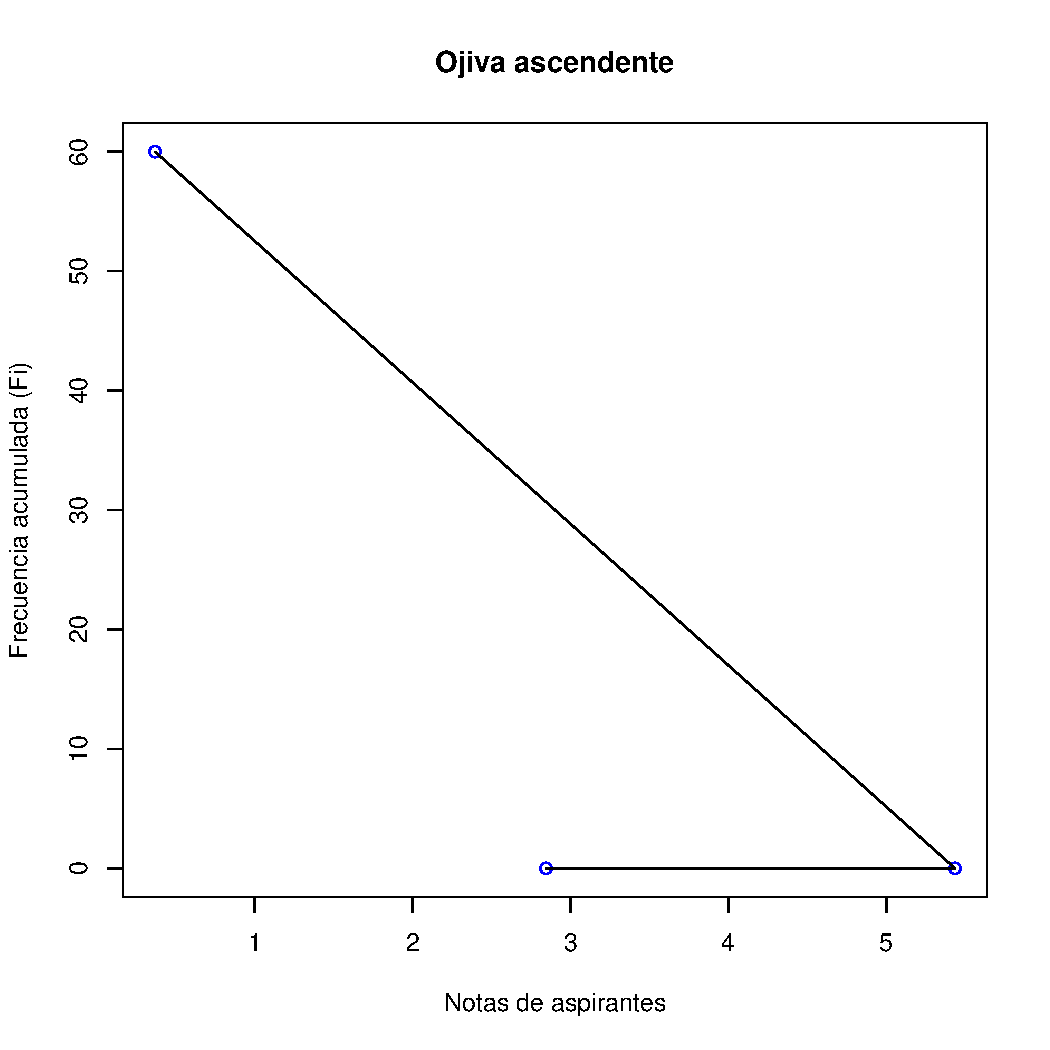
\includegraphics[width=\maxwidth]{figure/unnamed-chunk-19-1} 

\end{knitrout}

\item  Calcula los principales estad\'itico descriptivos de la variable
\begin{knitrout}
\definecolor{shadecolor}{rgb}{0.969, 0.969, 0.969}\color{fgcolor}\begin{kframe}
\begin{alltt}
\hlcom{# Calcula la moda, ya que el R no proporciona una funcion para eso.}
\hlkwd{options}\hlstd{(}\hlkwc{digits}\hlstd{=}\hlnum{4}\hlstd{)}
\hlkwa{for}\hlstd{(i} \hlkwa{in} \hlnum{1}\hlopt{:}\hlstd{k)}
  \hlkwa{if} \hlstd{(fi[i]} \hlopt{==} \hlkwd{max}\hlstd{(fi))} \hlkwa{break}\hlstd{()}
\hlkwa{if}\hlstd{(i} \hlopt{>} \hlnum{1}\hlstd{) moda} \hlkwb{<-} \hlstd{limites[i]}\hlopt{+}\hlstd{((fi[i]}\hlopt{-}\hlstd{fi[i}\hlopt{-}\hlnum{1}\hlstd{])}\hlopt{/}\hlstd{((fi[i]}\hlopt{-}\hlstd{fi[i}\hlopt{-}\hlnum{1}\hlstd{])}\hlopt{+}
 \hlstd{(fi[i]}\hlopt{-}\hlstd{fi[i}\hlopt{+}\hlnum{1}\hlstd{]) ))}\hlopt{*}\hlstd{a} \hlkwa{else} \hlstd{moda} \hlkwb{<-} \hlstd{limites[i]}\hlopt{+}\hlstd{(fi[i]}\hlopt{/}\hlstd{(fi[i]}\hlopt{+}
                          \hlstd{(fi[i]}\hlopt{-}\hlstd{fi[i}\hlopt{+}\hlnum{1}\hlstd{])))}\hlopt{*}\hlstd{a}
\hlstd{moda}
\end{alltt}
\begin{verbatim}
## to 
## NA
\end{verbatim}
\end{kframe}
\end{knitrout}

\begin{knitrout}
\definecolor{shadecolor}{rgb}{0.969, 0.969, 0.969}\color{fgcolor}\begin{kframe}
\begin{alltt}
\hlcom{# Calcula los cuartiles: Q1, Q2, Q3}

\hlstd{Q} \hlkwb{<-} \hlnum{1}\hlopt{:}\hlnum{3}
\hlkwa{for}\hlstd{(v} \hlkwa{in} \hlnum{1}\hlopt{:}\hlnum{3}\hlstd{)} \hlkwa{for}\hlstd{(i} \hlkwa{in} \hlnum{1}\hlopt{:}\hlstd{k)} \hlkwa{if} \hlstd{(Fi[i]} \hlopt{>} \hlstd{(v}\hlopt{*}\hlnum{25}\hlopt{*}\hlstd{n)}\hlopt{/}\hlnum{100}\hlstd{)}
\hlstd{\{}
  \hlstd{Q[v]} \hlkwb{<-} \hlstd{limites[i]}\hlopt{+}\hlstd{(((}\hlnum{25}\hlopt{*}\hlstd{v}\hlopt{*}\hlstd{n}\hlopt{/}\hlnum{100}\hlstd{)}\hlopt{-}\hlstd{Fi[i}\hlopt{-}\hlnum{1}\hlstd{])}\hlopt{/}\hlstd{fi[i])}\hlopt{*}\hlstd{a}
  \hlkwa{break}
\hlstd{\}}
\hlstd{Q}
\end{alltt}
\begin{verbatim}
## [1] 5.527 5.619 5.712
\end{verbatim}
\end{kframe}
\end{knitrout}
\end{enumerate}



\end{document}
